\iffalse
\documentclass[journal,12pt,twocolumn]{IEEEtran}
\usepackage{setspace}
\usepackage{gensymb}
\singlespacing
\usepackage[cmex10]{amsmath}
\usepackage{amsthm}
\usepackage{mathrsfs}
\usepackage{txfonts}
\usepackage{stfloats}
\usepackage{bm}
\usepackage{cite}
\usepackage{cases}
\usepackage{subfig}
\usepackage{longtable}
\usepackage{multirow}
\usepackage{enumitem}
\usepackage{mathtools}
\usepackage{tikz}
\usepackage{circuitikz}
\usepackage{verbatim}
\usepackage[breaklinks=true]{hyperref}
\usepackage{tkz-euclide} % loads  TikZ and tkz-base
\usepackage{listings}
\usepackage{color}    
\usepackage{array}    
\usepackage{longtable}
\usepackage{calc}     
\usepackage{multirow} 
\usepackage{hhline}   
\usepackage{ifthen}   
\usepackage{lscape}     
\usepackage{chngcntr}
\DeclareMathOperator*{\Res}{Res}
\renewcommand\thesection{\arabic{section}}
\renewcommand\thesubsection{\thesection.\arabic{subsection}}
\renewcommand\thesubsubsection{\thesubsection.\arabic{subsubsection}}

\renewcommand\thesectiondis{\arabic{section}}
\renewcommand\thesubsectiondis{\thesectiondis.\arabic{subsection}}
\renewcommand\thesubsubsectiondis{\thesubsectiondis.\arabic{subsubsection}}
\renewcommand\thetable{\arabic{table}}
% correct bad hyphenation here
\hyphenation{op-tical net-works semi-conduc-tor}
\def\inputGnumericTable{}                                 %%

\lstset{
%language=C,
frame=single, 
breaklines=true,
columns=fullflexible
}
%\lstset{
%language=tex,
%frame=single, 
%breaklines=true
%}

\begin{document}
\newtheorem{theorem}{Theorem}[section]
\newtheorem{problem}{Problem}
\newtheorem{proposition}{Proposition}[section]
\newtheorem{lemma}{Lemma}[section]
\newtheorem{corollary}[theorem]{Corollary}
\newtheorem{example}{Example}[section]
\newtheorem{definition}[problem]{Definition}
\newcommand{\BEQA}{\begin{eqnarray}}
\newcommand{\EEQA}{\end{eqnarray}}
\newcommand{\define}{\stackrel{\triangle}{=}}
\bibliographystyle{IEEEtran}
\providecommand{\mbf}{\mathbf}
\providecommand{\pr}[1]{\ensuremath{\Pr\left(#1\right)}}
\providecommand{\qfunc}[1]{\ensuremath{Q\left(#1\right)}}
\providecommand{\sbrak}[1]{\ensuremath{{}\left[#1\right]}}
\providecommand{\lsbrak}[1]{\ensuremath{{}\left[#1\right.}}
\providecommand{\rsbrak}[1]{\ensuremath{{}\left.#1\right]}}
\providecommand{\brak}[1]{\ensuremath{\left(#1\right)}}
\providecommand{\lbrak}[1]{\ensuremath{\left(#1\right.}}
\providecommand{\rbrak}[1]{\ensuremath{\left.#1\right)}}
\providecommand{\cbrak}[1]{\ensuremath{\left\{#1\right\}}}
\providecommand{\lcbrak}[1]{\ensuremath{\left\{#1\right.}}
\providecommand{\rcbrak}[1]{\ensuremath{\left.#1\right\}}}
\theoremstyle{remark}
\newtheorem{rem}{Remark}
\newcommand{\sgn}{\mathop{\mathrm{sgn}}}
\providecommand{\abs}[1]{\left\vert#1\right\vert}
\providecommand{\res}[1]{\Res\displaylimits_{#1}} 
\providecommand{\norm}[1]{\left\lVert#1\right\rVert}
\providecommand{\mtx}[1]{\mathbf{#1}}
\providecommand{\mean}[1]{E\left[ #1 \right]}
\providecommand{\fourier}{\overset{\mathcal{F}}{ \rightleftharpoons}}
\providecommand{\system}[1]{\overset{\mathcal{#1}}{ \longleftrightarrow}}
\newcommand{\solution}{\noindent \textbf{Solution: }}
\newcommand{\cosec}{\,\text{cosec}\,}
\providecommand{\dec}[2]{\ensuremath{\overset{#1}{\underset{#2}{\gtrless}}}}
\newcommand{\myvec}[1]{\ensuremath{\begin{pmatrix}#1\end{pmatrix}}}
\newcommand{\mydet}[1]{\ensuremath{\begin{vmatrix}#1\end{vmatrix}}}
\let\vec\mathbf
\def\putbox#1#2#3{\makebox[0in][l]{\makebox[#1][l]{}\raisebox{\baselineskip}[0in][0in]{\raisebox{#2}[0in][0in]{#3}}}}
     \def\rightbox#1{\makebox[0in][r]{#1}}
     \def\centbox#1{\makebox[0in]{#1}}
     \def\topbox#1{\raisebox{-\baselineskip}[0in][0in]{#1}}
     \def\midbox#1{\raisebox{-0.5\baselineskip}[0in][0in]{#1}}

\vspace{3cm}
\title{Optimization Assignment}
\author{Gautam Singh}
\maketitle
\bigskip

\begin{abstract}
    This document contains the solution to Question 4 of Exercise 2 in Chapter
    10 of the class 11 NCERT textbook.
\end{abstract}

\begin{enumerate}
  
    \solution 
    \fi
		We rewrite the problem as
    \begin{align}
        \min_{\vec{x}} h\brak{\vec{x}} &\triangleq \norm{\vec{x}-\vec{P}}^2 \\
        \textrm{s.t. } g\brak{\vec{x}} &\triangleq \vec{n}^\top\vec{x} - c = 0
        \label{eq:11/10/3/14/lagmul/lag-opt}
    \end{align}
    where
    \begin{align}
        \vec{P} = \myvec{-1\\3},\ \vec{n} = \myvec{3\\-4},\ c = 16
        \label{eq:11/10/3/14/lagmul/vals}
    \end{align}
    Define
    \begin{align}
        C\brak{\vec{x},\lambda} &= h\brak{\vec{x}} - \lambda g\brak{\vec{x}}
        \label{eq:11/10/3/14/lagmul/C-def}
    \end{align}
    and note that
    \begin{align}
        \nabla h\brak{\vec{x}} &= 2\brak{\vec{x}-\vec{P}} \\
        \nabla g\brak{\vec{x}} &= \vec{n}
        \label{eq:11/10/3/14/lagmul/diff-gh}
    \end{align}
    We are required to find $\lambda \in \mathbb{R}$ such that
    \begin{align}
        \nabla C\brak{\vec{x},\lambda} &= 0 \\
        \implies 2\brak{\vec{x}-\vec{P}} - \lambda\vec{n} &= 0
        \label{eq:11/10/3/14/lagmul/x-lambda}
    \end{align}
    However, $\vec{x}$ lies on the line \eqref{eq:11/10/3/14/lagmul/line}. Thus, from
    \eqref{eq:11/10/3/14/lagmul/x-lambda},
    \begin{align}
        \vec{n}^\top\brak{\frac{\lambda}{2}\vec{n}+\vec{P}} - c &= 0 \\
        \implies \lambda &= \frac{2\brak{c-\vec{n}^\top\vec{P}}}{\norm{\vec{n}}^2}
        \label{eq:11/10/3/14/lagmul/lambda-opt}
    \end{align}
    Substituting \eqref{eq:11/10/3/14/lagmul/lambda-opt} in \eqref{eq:11/10/3/14/lagmul/x-lambda}, the optimal
    point is given by
    \begin{align}
        \vec{Q} &= \vec{P} + \frac{\lambda}{2}\vec{n} \\
                &= \vec{P} - \frac{\vec{n}^\top\vec{P}-c}{\norm{\vec{n}}^2}\vec{n}
                \label{eq:11/10/3/14/lagmul/x-sol-lag}
    \end{align}
    Substituting from \eqref{eq:11/10/3/14/lagmul/vals},
    \begin{align}
        \lambda = \frac{62}{25},\ \vec{Q} = \frac{1}{25}\myvec{68\\-49}
        \label{eq:11/10/3/14/lagmul/sol}
    \end{align}
    To find $\vec{Q}$ graphically, we use constrained gradient descent, with
    learning rate $\alpha = 0.01$. The results are shown in Fig.
    \ref{fig:11/10/3/14/lagmul/gd-lag}, plotted using the Python code.
    \begin{figure}[!ht]
        \centering
        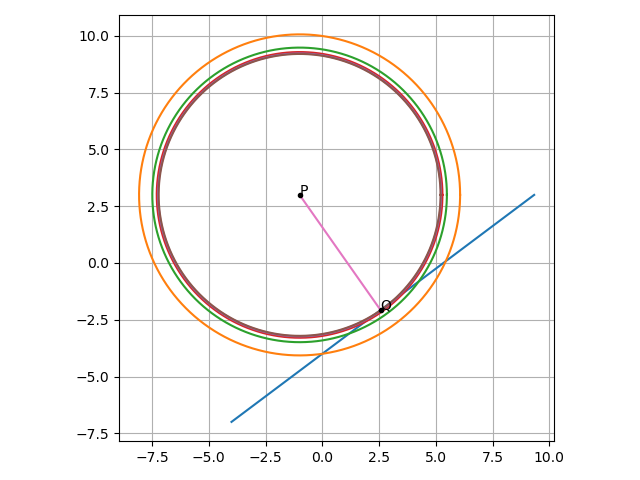
\includegraphics[width=\columnwidth]{11/10/3/14/lagmul/figs/gd_lagrange.png}
        \caption{Constrained gradient descent to find optimal $\vec{Q}$.}
        \label{fig:11/10/3/14/lagmul/gd-lag}
    \end{figure}
\textit{Constrained gradient descent} is a method of optimizing the cost function
subject to some constraints, represented as follows.
\begin{align}
    \max_{\vec{x}}f\brak{\vec{x}} \label{eq:11/10/3/14/lagmul/cgd-cost} \\
    \textrm{s.t. } g\brak{\vec{x}} = 0
    \label{eq:11/10/3/14/lagmul/cgd-constr}
\end{align}
Unlike the unconstrained version, one cannot move in the negative direction of the
gradient vector of $f\brak{\vec{x}}$. However, we must move along the constraint in
\eqref{eq:11/10/3/14/lagmul/cgd-constr}.

The algorithm terminates when the gradient vector of $f$ is parallel to the normal 
vector of $g$ at that point. Mathematically, at an optimum $\vec{x_o}$,
\begin{align}
    \nabla f\brak{\vec{x_o}} = \lambda\nabla g\brak{\vec{x_o}}
    \label{eq:11/10/3/14/lagmul/cgd-cond}
\end{align}
where $\lambda \in \mathbb{R}\setminus\cbrak{0}$. Observe that \eqref{eq:11/10/3/14/lagmul/cgd-cond}
may be rewritten as
\begin{align}
    \nabla C\brak{\vec{x},\lambda} = \nabla \brak{f\brak{\vec{x}}-\lambda g\brak{\vec{x}}} = 0
\end{align}
which is analogous to the method of Lagrangian multipliers.
